\subsection{\label{subsection:fuzzy-selection}Selection}
The selection operator is defined analogously as the crisp selection operator given in Definition \ref{def:crisp-selection} and the formal specification given by equation \eqref{eq:selection}. 
%In order to distinguish the possibilistic selection from the crisp selection, the possibilistic operators will be written with the superscript FT.


\begin{definition}
\label{def:poss-selection}
 Consider the elements in definition \ref{def:fuzzy-temporal-relation}.
The selection operator $\tilde\sigma^{T}$ returns a subset of tuples that fulfill a set of constraints $P$ from an instance $r$ of the relation $R$. The set of constraints is usually a boolean combination of atomic constraints. The selection operator is noted as follows:
\end{definition}

\begin{equation}
 \label{eq:poss-selection}
\tilde\sigma^{\mbox{T}}_{P} \left( r \right)
\end{equation}

Where $r \in R$ is the relation, and $P$ is the selection formula. 


In the possibilistic model, the main modification is that the selection predicate $P$ is not a boolean function. The selection predicate $P$ returns a satisfaction degree (in the unit interval). 
The selection formula has the same appearance than the crisp selection formula in equation \eqref{eq:selection_formula}:
\begin{equation}
 \label{eq:fuzzy-selection_formula}
P = \left \lbrace Q, Q^{T}\right \rbrace
\end{equation}

In this case, in order to evaluate both, where  $Q$ and $Q^{T}$ could be fuzzy or crisp predicates, it is necessary to define the evaluation functions for both $Q$ and $Q^{T}$. We will illustrate the possibilistic evaluation of $Q$. The possibilistic evaluation of $Q^T$ is analogous. First of all, consider a boolean function $\bool:\Boolean^{n}  \rightarrow \Boolean$. The evaluation function for the constraints in $Q$  is given by:

\begin{equation}
 \label{eq:evaluation-function}
\lambda : Q \rightarrow \Boolean : \lambda (Q) \rightarrow \bool \left(q_{a_1}  \theta \mbox{ val }, \ldots, q_{a_n}  \theta \mbox{ val } \right)
\end{equation}

Now, the uncertainty about the evaluation of $Q$ and a boolean function $\bool:\Boolean^{n}  \rightarrow \Boolean$ is given by:

\begin{equation}
 \label{eq:evaluation-lambda-function}
\pi_{\lambda \left(Q \right)} = \tilde{\bool} \left(\pi_{q_{a_1}  \theta \mbox{ val }}, \ldots, \pi_{q_{a_n}  \theta \mbox{ val }} \right)
\end{equation}




% The temporal constraints, $Q^t$ are provided in a similar way. The main difference is that, instead of comparations like $\left \lbrace =, \neq, <, \leq, >, \geq \right \rbrace$, we use the allen's relations. Hence, the representation of the temporal constraints is expressed as follows:
% 
% \begin{equation}
% \label{eq:temporal-constratins}
% Q^{t} = \left \lbrace q_{v_1}  ar \mbox{ val }, \ldots, q_{v_n}  ar \mbox{ val } \right \rbrace
% \end{equation}
% Here, $ar$ is one of the thirdteen Allen's relations (equal, before, overlaps, starts, finishes, meets, during) and their respective reverses.


\subsubsection{Query Evaluation}
In fuzzy querying of regular (relational) databases, the modelling of query satisfaction is a matter of degree. Usually, the evaluation of the query requirements for a record results in a satisfaction degree $s$, where $s$ lies in $\left[0,1\right]$, where 0 denotes total dissatisfaction and 1 denotes complete satisfaction. In crisp querying, the evaluation of query requirements for a record results in the accepting or rejecting of the record as a part of the result set. This can be modelled using satisfaction degrees, by assigning rejection a degree of $0$ and acceptance a degree of $1$ and not using any other value in $\left[0,1\right]$.

The evaluation of the predicate $P = \left( Q, Q^T \right)$, is now handled as follows. For each record $r$ in the database, with the valid-time notion of $r$ being specified by a PVP $J$, two events happen independently:


\begin{itemize}
\item
The preferences expressed in $Q$ are evaluated, resulting in a satisfaction degree denoted here $e_{Q}(r)$. The presented model accepts any sound way of calculating this evaluation, as long as $e_{Q}(r) \in \left[0,1\right]$. 
\item
Depending on the Allen Relation selected ($\AR$), a specific set of ill-known constraints is considered. The possibility and necessity that $r$ fulfills all these constraints are calculated using formulas based on equations \eqref{ill-known-pos} respectively \eqref{ill-known-nec} and aggregated using the $\min$ operator. 
\end{itemize}



\subsubsection{Aggregation and Ranking}
In order to present the results to the user, a crude ranking method is used: for every record $r$, the sum of $\Pos_{Q^{time}}(r)$ and $\Nec_{Q^{time}}(r)$ gives an evaluation score $e'_{Q^{time}}(r)$ in interval $\left[0,2\right]$. Because necessity cannot exceed $0$ unless possibility is $1$, this gives a natural ranking score. Some authors ~\cite{Bosc2010a} mentioned before that the possibility and necessity measures result in a total order in the set of events.  This $e'_{Q^{time}}(r)$ is then rescaled to the unit interval, resulting in $e_{Q^{time}}(r)$. The final ranking $e_{final}(r)$ is now given by a convex combination:


\begin{equation}
\label{eq:convex-comb}
e_{final}(r)\ =\ \omega*e_{Q}(r)\ +\ (1-\omega)*e_{Q^{time}}(r), \omega \in \left[0, 1 \right]
\end{equation}

The use of this convex combination allows a record to make up for a low score for the temporal constraint by a good score for the non-temporal constraint (or vice versa). Changing $\omega$ also allows granting the temporal constraint more weight with respect to the non-temporal constraint (or vice versa).

\begin{example} 
Consider the example relation $c \in C$ given in Table \ref{tb:car-models} describing car models, containing general attributes (model name, manufacturer, car segment) and one PVP  describing the approximate period of time during which the car model was sold. In this example, the value for $D$ is stored in \emph{yyyy} format and $a$ and $b$ are represented by an integer. The ID field identifies a car model while the field Instance ID (IID) identifies the instance for a car model, thus a car model in a certain state.
\end{example}


\begin{table}[h]
\centering
\caption{Example database, instance $c \in C$}
\vspace{2mm}
\begin{tabular}{c c c c c c c}
\hline
ID & IID & Segment & Manufacturer & Name & Start & End  \\ [0.5ex]
\hline
001 & 1 & B & Peugeot & 205 & [1985,2,3] & [1997,2,1] \\
002 & 1 & C & Peugeot & 305 & [1977,2,2] & [1989,2,3] \\
003 & 1 & B & Citroen & C2 & [2001,1,1] & [2005,1,1] \\
001 & 2 & B & Peugeot & 206 & [2000,1,2] & [2011,2,1] \\
001 & 3 & B & Peugeot & 207 & [2006,1,1] & [2011,1,1]\\
\hline
\end{tabular}
%\vspace{10pt}
\label{tb:car-models}
%\vspace{-30pt}
\end{table}

Consider the following query:
\begin{center}
\emph{The user wants to obtain a list of models from segment B, sold by manufacturer Peugeot before the Citroen C2.}\\
\end{center}

Using the introduced notations in \eqref{eq:poss-selection},\eqref{eq:fuzzy-selection_formula}, the query is translated to: 
\begin{equation}
\tilde \sigma^{\mbox{T}}_{\left \lbrace Q, Q^T\right \rbrace} \left( c \right)\
\end{equation}

The query constraints are the following:

\begin{align}
Q & = \left(c.Segment =  B\right) \wedge \left(c.Manufacturer = Peugeot\right)\\
Q^{T} & = c.\left[S, E \right] \mbox{Before} \left[2001,1,1\right], \left[2005,1 ,1 \right]
\end{align}


\begin{table}[ht]
\caption{Result table and ranking}
\centering
\begin{tabular}{c c c c c c c}
\hline
ID & IID &  $\Pos_{Q^{T}}$ & $\Nec_{Q^{T}}$ & $e_{Q^{T}} (rescaled)$ & $Q$ & $e_{final}$ ($\omega=0.5$) \\ [0.5ex]
\hline
001 & 1 & 1 &  1 & 1 & 1 & 1 \\
002 & 1 & 1 & 1 & 1 & 0.5 & 0.75 \\
003 & 1 & 1 & 0.5 & 0.75 &0 & 0.375\\
001 & 2 & 1 & 0 & 0.5 &1 & 0.75 \\
001 & 3 & 0 & 0 & 0 &1 & 0.5\\
\hline
\end{tabular}
\label{tb:results}
\end{table}

Table \ref{tb:results} shows a natural and gradual ranking for the results. The last record, (ID 001, IID 3) shows also that with $\omega$ = 0.5 both temporal and regular criteria have the same importance.

\subsection{\label{subsection:fuzzy-cartesian-product}Cartesian Product}

In this subsection we are going to extend the crisp version of the temporal cartesian product to deal with ill-known time intervals. First of all, we need to define the ill-known counterpart functions of the previously defined \emph{intersects, first, last, OvIn}.

\begin{definition}
 \label{def:ik-intersects}
Two ill-known time intervals intersect if one or both of the before and after relationships do not hold. Consider $I = \left[I_s, I_e \right]$ and $J = \left[J_s, J_e \right]$ be two ill-known time intervals with $I_s, J_s$ the starting ill-known points and $I_e, J_e$ the ending ill-known points of the intervals. Let the following ill-known constraints:
\begin{align}
 \label{eq:ik-intersects}
C_1 &=& \left(<, I_s \right)  \\
C_2 &=& \left(=, J_s \right) \\
C_3 &=& \left(<, J_s \right) \\
C_4 &=& \left(=, I_s \right) \\
\mbox{Intersects}\left(I, J\right) &=& \left \lbrace \neg \left(C_1 \wedge C_2 \right) \vee  \neg \left( C_3 \wedge C_4 \right)  \right \rbrace \\
\nonumber
&=& \left \lbrace \neg \left( \left(C_1 \wedge C_2 \right) \wedge \left(C_3 \wedge C_4 \right)  \right)\right \rbrace
\end{align}
\end{definition}


\begin{definition}
 \label{def:ik-last}
Last$\left(I_n, J_m \right)$. Given two ill-known points $I_n$ and $I_m$, the last operator is a combination of the following ill-known constraints:
\begin{align}
 \label{eq:il-last}
C_1 &=& \left(>, I_n \right) \\
C_2 &=& \left(=, J_m \right) \\
C_3 &=& \left(>, J_m \right) \\
C_4 &=& \left(=, I_n \right) \\
\mbox{Last}\left(I_n, J_m \right) &=& \left(C_1 \wedge C_2  \right) \vee \left(C_3 \wedge C_4 \right)
\end{align}
\end{definition}

Analogously, the first operator is defined as follows.
\begin{definition}
 \label{def:ik-first}
First$\left(I_n, J_m \right)$. Given two ill-known points $I_n$ and $I_m$, this operator is a combination of the following ill-known constraints:
\begin{align}
 \label{eq:ik-first}
C_1 &=& \left(<, I_n \right)\\
C_2 &=& \left(=, J_m \right)\\
C_3 &=& \left(<, J_m \right) \\
C_4 &=& \left(=, I_n \right) \\
\mbox{First}\left(I_n, J_m \right) &=& \left(C_1 \wedge C_2  \right) \vee \left(C_3 \wedge C_4 \right)
\end{align}
\end{definition}

Now it is possible to define the function overlapping interval for the ill-known case.

\begin{definition}
 \label{def:ik-overlapping-interval}
Given two ill-known time intervals $I$ and $J$, this function returns an overlapping interval from the original two intervals. It is necessary to define two ill-known constraints:

\begin{align}
 \label{eq:ilc-smaller-than}
C_1 &=& \left(\leq,\mbox{First}\left(I_e, J_e \right)\right) \\
C_2 &=& \left(=, \mbox{Last}\left( I_s, J_s \right)\right)
\end{align}



\begin{equation}
 \mbox{OvInt}\left(I, J \right) = 
\begin{cases}
\left[\mbox{Last}\left( I_s, J_s \right), \mbox{First}\left(I_e, J_e \right) \right] & \mbox{ if } C_1 \wedge C_2 \neq 0.  \\
\emptyset & \mbox{ otherwise } 
\end{cases}
\end{equation}
\end{definition}

Finally, the temporal cartesian product for ill-known time intervals is defined as follows.

\begin{definition}
 \label{def:temporal-cartesian-product-ik}Temporal cartesian product.Consider the elements in definition \ref{def:generalized-fuzzy-temporal-relation}.
The temporal cartesian product is notated $r \times^{FT} s$ and is given by the following equation:
\begin{align}
 \label{eq:ik-temporal-cartesian-product}
r \tilde \times^{T} s = \left \lbrace z^{\left(n+m+2\right)}  | \exists x \in r, \exists y \in s \right. \\
\nonumber
\mbox{intersect}\left(x[S, E], y[S, E] \right) > 0 \wedge \\
\nonumber
z\left[A\right] = x\left[A\right] \wedge z\left[B\right] = y \left[B \right] \wedge \\
\nonumber
\left.  z\left[S, E \right] = \mbox{OvInt}\left(x\left[S, E\right], y\left[S, E\right] \right) \wedge z\left[S, E\right] \neq \emptyset  \right \rbrace
\end{align}
\end{definition}

The temporal cartesian product by ill-known constraints is illustrated in the following example.
\begin{example}
 \label{ex:temporal-ill-known-constraint-ik}
Consider a ill-known version of the employee's database, as illustrated by tables \ref{table:ill-known-employees} and \ref{table:ill-known-addresses}
\end{example}

\begin{table}[h]
\centering
\caption{Relation for the employees with an ill-known valid-time interval.}
\vspace{2mm}
\begin{tabular}{c c c c c c }
\hline
ID & Job & Works for & Start & Finish \\ \hline
1 & Prof. & 4 & $\left[5, 1, 1 \right]$ & $\left[10, 1, 1 \right]$ \\
2 & Tech. & 4 & $\left[3, 1, 1 \right]$ & $\left[7, 1, 1 \right]$ \\
\hline 
\end{tabular}
\label{table:ill-known-employees}
\end{table}

\begin{table}[h]
\centering
\caption{Relation for the addresses with an ill-known valid-time interval.}
\vspace{2mm}
\begin{tabular}{c c c c }
\hline
ID & Address & Start & Finish \\ \hline
1 & C/ Camino de Ronda & $\left[1, 1, 1 \right]$ & $\left[12, 1, 1 \right]$ \\
2 & C/ Recogidas &  $\left[1, 1, 1 \right]$ & $\left[5, 1, 1 \right]$ \\
\hline 
\end{tabular}
\label{table:ill-known-addresses}
\end{table}


\begin{table}[h]
\centering
\caption{Intermediate calculations for the temporal cartesian product.}
\vspace{2mm}
\begin{tabular}{c c c c c }
\hline
r.id & s.id &  intersect$\left(x\left[T\right], y\left[T\right]\right)$ &  Last$\left( I_s, J_s \right)$ & First$\left(I_e, J_e \right)$  \\ \hline
1 & 1 & 1 & $\left[5, 1, 1 \right]$ & $\left[10, 1, 1 \right]$ \\
1 & 2 & 1 & $\left[5, 1, 1 \right]$ & $\left[5, 1, 1 \right]$ \\
2 & 1 & 1 & $\left[3, 1, 1 \right]$ & $\left[7, 1, 1 \right]$ \\
2 & 2 & 1 & $\left[3, 1, 1 \right]$ & $\left[5, 1, 1 \right]$ \\
\hline 
\end{tabular}
\label{table:example-ik-cartesian-product}
\end{table}


\subsubsection{\label{sec:poss-join}Join}
The possibilistic join operator $\tilde \Join$ builds a new fuzzy temporal relation from two given relations, namely $r \in R$ and $s \in S$. This new relation is a set with all the possible combinations of tuples in both $r$ and $s$. It is usually noted as $r \tilde \Join_{a \theta b} s$ and called (theta) join, where $a,b$ are attributes from $r$ and $s$ respectively and $\theta$ a relational operator. The possibilistic temporal join definition is based on the temporal cartesian product.

\begin{definition}
 \label{def:poss-temporal-theta-join}
Temporal theta join. Let $r$ and $s$ be two  instances of relations $R, S$ respectively. Then the temporal theta join is defined as follows:
\begin{equation}
 \label{eq:poss-temporal-theta-join}
r \tilde \Join_{a \theta b}^{T} s= \sigma_{a \theta b} \left(r \tilde \times^{T} s \right)
\end{equation}

\end{definition}


% \begin{figure}
%  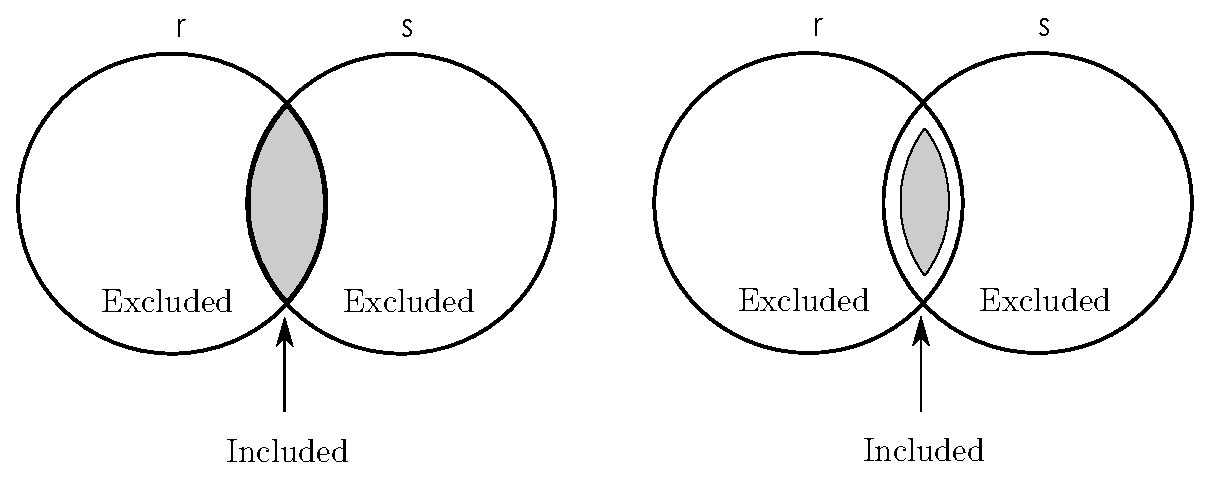
\includegraphics[scale=0.60]{graphs/innerjoin.eps}
% \caption{\label{fi:innerjoin} Comparison between the relational (non-temporal) inner join (left graph) and the temporal inner join (right graph).}
% \end{figure}


% 
% Figure \ref{fi:innerjoin} compares the relational inner join with respect to the temporal inner join. The right graph illustrates the temporal case. It is clear that the temporal inner join is a subset or is equal to the relational inner join.

% \subsubsection{\label{subsec:poss-Equijoin}Equijoin}
% The equijoin operator for relational databases enforces equality between specified subsets of the attributes of the relations. Then, the temporal equijoin operator is defined as the possbilistic temporal join operator.
% 
% \begin{definition}
%  \label{def:poss-equijoin}
% Equijoin. Let $R$ and $S$ be two relations and $r, s$ be the instances of each relation respectively. $A , B$ are the sets of the attributes for the relations $R$ and $S$ respectively. And let $A' \subseteq A$ and $B' \subseteq B$. Then, the temporal equijoin is defined as follows:
% \begin{equation}
%  \label{eq:poss-equijoin}
% r \Join_{r\left[A' \right] = s\left[B' \right]}^{FT} s =  \sigma^{FT}_{r\left[A' \right] = s\left[B' \right]} \left(r \times^{FT} s \right)
% \end{equation}
% \end{definition}
% 
% 
% \subsubsection{\label{subsubsec:poss-temporal-equijoin}Temporal Equijoin}
% The temporal equijoin is an equijoin operator in which the subset of attributes in the equijoin condition, are part of the primary key. Hence, the operator is defined as follows:
% 
% \begin{definition}
% \label{def:poss-temporal-equijoin}
% Temporal equijoin ($r \mbox{ TE-join }^{FT} s$). Let $R, S$ be two relations and $r, s$ the instances of each relation respectively. Consider that $PK$ is the primary key of both relations. The temporal equijoin operator is defined as follows:
% \begin{equation}
%  \label{eq:poss-temporal-equijoin} 
% r \mbox{ TE-join }^{FT} s \equiv r \Join_{r\left[PK\right] = s\left[PK\right]}^{FT} s
% \end{equation}
% \end{definition}
% 
% \subsubsection{\label{subsec:poss-natural-join}Natural Join}
% The temporal natural join is a temporal equijoin on identically named attributes.
% 
% \begin{definition}
%  \label{def:poss-temporal-natural-join}
% Temporal natural join. Consider the following relations $R = \left(A_1, \ldots, A_n, C_1, \ldots, C_k, S, E \right)$ and $S = \left(B_1, \ldots, B_m, C_1, \ldots, C_k, S, E \right)$. Let $r,s$ be instances of $R, S$ respectively. The temporal natural join is defined as follows:
% \begin{equation}
%  \label{eq:poss-temporal-natural-join}
% r \Join^{FT} s = r \Join^{FT}_{r\left[C_1\right] = s\left[C_1\right] \wedge \ldots \wedge r\left[C_k\right] = s\left[C_k\right]} s
% \end{equation}
% \end{definition}

% \todo[caption={outer-joins}]{Still have to define the outer joins implementation...}
% \subsubsection{\label{subsec:poss-outer-joins}Outer Joins}
% 
% 
% % \begin{figure}
% %  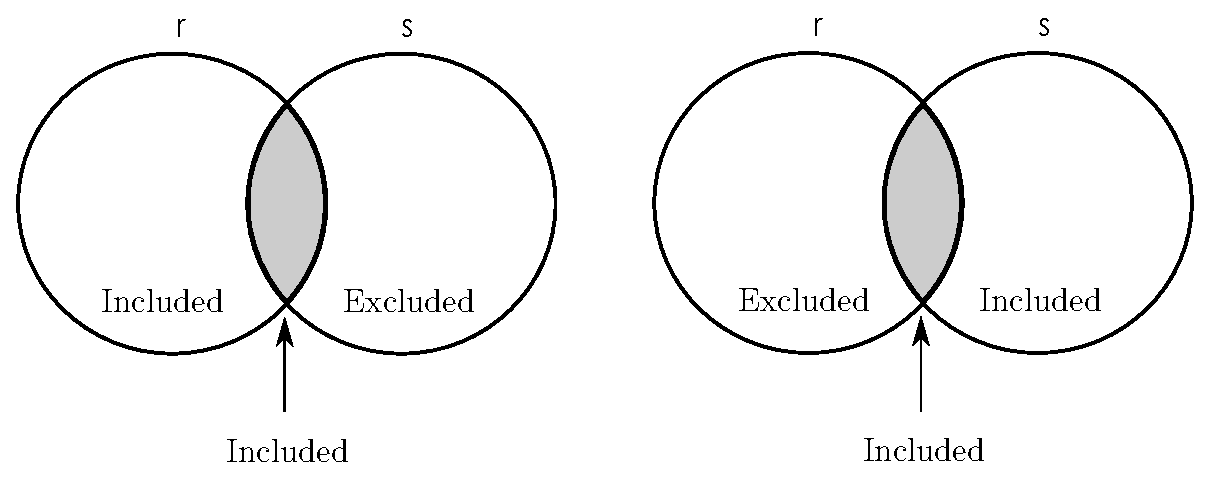
\includegraphics[scale=0.60]{graphs/outerjoin.eps}
% % \caption{\label{fi:outerjoin} Comparison between a left outer join (left graph) and a right inner join (right graph).}
% % \end{figure}


\subsection{Selection}
\subsection{Projection}
\subsection{Cartesian Product}
\subsection{Union}
\subsection{Difference}
\subsection{Intersection}
\subsection{Join}
\subsection{Division}